\documentclass[book.tex]{subfiles}
\begin{document}
The game ended up a big hit. Sales were so good the six original episodes were not enough to satisfy players:\\
\par
\begin{itemize}
\item Episode 1: Escape from Wolfenstein\\
\item Episode 2: Operation: Eisenfaust\\
\item Episode 3: Die, Fuhrer, Die!\\
\item Episode 4: A Dark Secret\\
\item Episode 5: Trail of the Madman\\
\item Episode 6: Confrontation\\
\end{itemize}
Sequels and port to other machines made business sense. id Software ended up developing some and contracting others. With one notorious port (iOS) coming out almost 20 years later in 2009.

\section{Spears of Destiny}
Released on September 18, 1992 Spears Of Destiny used the same game engine but with new graphics, music and levels. It is a prequel to the adventures of wolf hero: B.J. Blazkowicz. It consist of one additional episode of 21 levels.\\
   \par
\begin{figure}[H]
\centering
 \fullimage{spears_of_destiny_intro.png}
 \end{figure}
 \par
 The game resued Wolfenstein 3D engine, allowing a part of the team to release a second title while an other part of the team worked on the next technology to power DOOM. The title is nonetheless innovative since it introduces huge transparent sprites to simulate vegetation and also tries to break away from the orthogonal world with clever map design:
    \par
\begin{figure}[H]
\centering
 \fullimage{spears_of_destiny_play.png}
 \end{figure}
 \par


   \par
\begin{figure}[H]
\centering
 \fullimage{spears_of_destiny_creative_map.png}
 \end{figure}
 \par


 SOD features a copy protection mechanism: A set of random question which could only be answered with the game manual:\\
    \par
\begin{figure}[H]
\centering
 \fullimage{spears_of_destiny_copy_protection.png}
 \end{figure}
 \par
 An easter egg is hidden here. A serie of word are always a valid answer. Amond them "Joshua", a reference to 1983 movie WarGames:\\
    \par
\begin{figure}[H]
\centering
 \fullimage{spears_of_destiny_easter_egg.png}
 \end{figure}
 \par



Trivia: Angel of Death looked like a demon and was a good insight into what would come next: Doom.




It was essentially a mod of Wolfenstein 3D. SOD helps to put things into perspective when it comes to being open source and allow people to figure out the file formats. SOD may not have sold as well had the game been open.\\
No a shareware version  but  2-level playable demo was distributed\\
Lost Episodes, Each of these, consists of 21 levels. New level textures, new enemies, and new appearances for old enemies. Published by FormGen Corporation in May 1994.''
\\
\section{Mission Pack}
Mission Packs(released by FormGen Corporation in May 1994, resemble many fan-made mods a.k.a: Lost Episodes):\\
Mission 2: Return to Danger\\
Mission 3: Ultimate Challenge\\



\section{Port: Super Nintendo}
The port to Super Nintendo was done during the development of Doom. id Software ported the game in three weeks after the guy in charge of porting Wolfenstein failed to deliver.

 \begin{fancyquotes}
Disaster Struck.\\
\par
We all had to stop working on Doom. The Super Nintendo version that we had gotten a guy to work on was not finished. And Imagineer was not pleased. It had been since the summertime so it had been about nine months and they hadn't head anything from us. That guy was working on the port and we could not get ahold of the guy. It was a nightmare situation. We could not get it done with somebody else. So, basically, we stopped working on Doom and ported Wolfenstein to the Super Nintendo. The whole team jumped on it. It tooks us like three weeks to just blast out the port. And that is including all rats in there and green blood.

The whole team jumped on it.
\\
\textbf{John Romero - Programmer}
\end{fancyquotes}

\par
\begin{figure}[H]
\centering
 \fullimage{wolf3d_snes_box.jpg}
 \end{figure}
 \par


\begin{fancyquotes}
    When I ported Wolf to the SNES, the ray casting performance cost was too much, so I had to make a new wall span renderer.  Learning about BSP trees allowed me  to much more accurately resolve the culling challenges, and it worked out ok, leading the way to the Doom renderer.\\
\\
Many years later, I made a very similar programming tradeoff for the mobile BREW version of Doom RPG.  The J2ME (java) Doom RPG looked like Wolfenstein, with a tile map world, textured walls, and solid color floor and ceiling, but it was done with a quite nice wall span renderer.  I had learned a thing or two since writing Wolf.  For the ARM native code BREW version, I wanted to add texture mapped floors and ceilings with per-tile texture choices.  I turned the tile maps into polygon windings and started writing a full texture mapped clipped polygon rasterizer for them, but I only had a couple days to work on the mobile renderer, and it became clear that I wasn’t going to be able to deliver a really solid implementation in that time.\\
 \\
The solution was to sacrifice performance for implementation simplicity.  Instead of trying to fill in just the empty pixels around the walls with floor / ceiling textures, I completely textured the entire screen with floor and ceiling textures before drawing the walls on top of them.  With floor / ceiling symmetry and fixed texture sizes, it was pretty fast even with per-pixel tile map lookup, but most importantly it was rock solid, crack free, and completed in the window of time I had allotted to it.\\
\\
\textbf{John Carmack - Programmer}
\end{fancyquotes}


\par
\begin{figure}[H]
\centering
 \fullimage{wolf3d_snes.png}
 \caption{Extremely low resolution during 3D scene: 125x125! (but the HUB and weapon are higher resolution which helps a little.)}
 \end{figure}
 \par


\section{Port: Jaguar}
The jaguar port was release in 1994 and it was the only other port (along with the SNES) made by id Software. It was the only port able to reach 60 frames per seconds. It was unique for having graphics in a resolution much superior to the PC release, and bilinear filtering. It also introduced two new weapons: the Flamethrower and Rocket Launcher:\\
\par

The console was a mix of powerful components with severe bottleneck: 
\bu{Trivia :} The Jaguar Chain Gun uses Doom's chaingun graphic as a base.\\
\par
\begin{fancyquotes}
The memory, bus, blitter and video processor were 64 bits wide, but the processors (68k and two custom risc processors) were 32 bit.\\
\\
The bliter could do basic texture mapping of horizontal and vertical spans, but because there wasn't any caching involved, every pixel caused two ram page misses and only used 1/4 of the 64 bit bus. Two 64 bit buffers would have easily tripled texture mapping performance. Unfortunate.\\
\\
It could make better use of the 64 bit bus with Z buffered, shaded triangles, but that didn't make for compelling games.\\
\\
It offered a usefull color space option that allowed you to do lighting effects based on a single channel, instead of RGB.\\
\\
The video compositing engine was the most innovative part of the console. All of the characters in Wolf3D were done with just the back end scalar instead of bliting. Still, the experience with the limitations and hard failure cases of that gave me good ammunition to rail against microsoft's (thankfully aborted) talisman project.\\
\\
The little risc engined were decent processors. I was surprised that they didn't use off the shelf designs, but they basically worked ok. They had some design hazards (write after write) that didn't get fixed, but the only thing truly wrong with them was that they had scratchpad memory instead of caches, and couldn't execute code from main memory. I had to chunk the DOOM renderer into nine sequentially loaded overlays to get it working (with hindsight, I would have done it differently in about three...).\\
\\
The 68k was slow. This was the primary problem of the system. You options were either taking it easy, running everything on the 68k, and going slow, or sweating over lots of overlayed parallel asm chunks to make something go fast on the risc processors.\\
\\
That is why playstation kicked so much ass for development -- it was programmed like a single serial processor with a single fast accelerator.\\
\\
If the jaguar had dumped the 68k and offered a dynamic cache on the risc processors and had a tiny bit of buffering on the blitter, it could have put up a reasonable fight against sony.\\
\\
\textbf{John Carmack - Programmer (March 4th, 2000)}
\end{fancyquotes}

\par
\begin{figure}[H]
\centering
 \fullimage{jaguar_port_cover.jpg}
\end{figure}
\par
\begin{figure}[H]
\centering
 \fullimage{jaguar_port_gatling.png}
\end{figure}
\par

\begin{figure}[H]
\centering
 \fullimage{jaguar_port_flamethrower.png}
\end{figure}









\section{Port: PC-98}
Essentially Japanese port. Explain the source code diff packages.








\section{Port: 3DO}
Because the 3DO port of Wolfenstein 3D was developed by the same company as the Macintosh port, the two games are nearly identical. They both feature higher resolution graphics, an in-game map, more weapons, and superior audio. However, unlike the original DOS version, the 3DO lacks rotating sprites, so enemies are always looking at you, making it impossible to sneak up on them.\\



talk about 3DO port: http://www.vgmpf.com/Wiki/index.php?title=Wolfenstein\_3D\_(3DO)\\


\section{Port: XBox360 and Playstation3}

\begin{fancyquotes}
I also had to make one last minute hack change to the original media — the Red Cross organization had asserted their trademark rights over red crosses (sigh) some time after we released the original Wolfenstein 3D game, and all new game releases must not use red crosses on white backgrounds as health symbols.  One single, solitary sprite graphic got modified for this release.
\\
\textbf{John Carmack - Programmer (Mar 04, 2000)}
\end{fancyquotes}
\section{Port: Macintosh}

Published with authorization

Unlike newer games (Doom, Unreal, etc) the Macintosh version is not just a port (exact translation) of the PC version. The levels and the game engines are actually quite different. Thus, you can not use levels and mods for one version with the other version.\\
\\
\subsection{Levels}

The first major difference is the level design. While the PC version contains 6 episodes with each episode containing 10 levels (1 of those is a hidden bonus level), the Macintosh version (reffered to as the 2nd Encounter) contains 30 levels with no divisions into episodes. The Mac version is divided into floors, but you can not start on a specific floor and every floor has a different amount of levels. A 3rd Encounter was later released for Macintosh containing 60 more levels which were supposed to make up episodes 2 to 6.\\
Obviously, the number of levels aren't the same but this doesn't necessarily mean that the Macintosh version is giving you more. Many of the levels are similar, but the Macintosh levels are usually much less intricate and much shorter. This is apparent in the first level where the path to the exit is exacly the same in both versions, but the PC version contains many more possible side-trips and many more rooms. Other levels in the games are completely different. Basically, the 2 games play extremely differently and offer unique experiences.

\subsection{Game Engine}
Another major difference is in the game engines. At first glance, the Macintosh engine, which is 2 years newer, seems to be the more advanced. The graphics in the Macintosh version are much sharper, clearer, and better looking at twice the resolution of the PC graphics. Also, the game takes up a slightly larger portion of the screen and the sounds are much higher quality in the Macintosh version.\\
However, the enemies in the Macintosh version are only 2D sprites whereas the enemies in the PC version are 3D sprites. This means that the Macintosh enemies only have 1 side, a front side, and thus, they are always facing you. In contrast, the PC enemies have 8 sides, making for much more realist play; in the PC version, it is possible to sneak up behind guards and kill them before they see you - something that can't be done in the Macintosh version.\\
\\
The enemies in the PC version also offer an extra level of realism by being able to patrol an area. In the Macintosh version, the enemies will just stand in one spot until they see you or hear you; in the PC version, enemies will stand in place or patrol an area until they see or hear you. These differences make the PC version's game engine more advanced despite being 2 years older.\\

\subsection{Weapons, Items, and Enemies}

Several other difference worth noting include the addition of 2 extra weapons in the Macintosh version: the flamethrower and the rocket launcher. Those two weapons and some other items (bullet crates, flame thrower and rocket ammo, backpacks) are not found in the PC version.
Also, some other pick-ups and dropped items are different. For example, in the PC version, dropped clips give 4 ammo and other clips give 8 ammo; in the Macintosh version, all clips give 5 ammo. Also, picking up treasure in the PC version adds to your score (40000 points gets you an extra life); in the Macintosh version, picking up treasure increases your item count by one until you get an extra life at 50 items.

Other differences include an additional enemy, the Flying Hitler, in the PC version and different bosses in the 2 versions (see the enemies and bosses pages); the Mac version actually uses some bosses from Wolfenstein 3D and some bosses from Spear of Destiny.

\subsection{Miscellaneous}

Yet another difference is that changing the difficulty level in the Macintosh version only affects the damage taken and starting ammo whereas in the PC version it affects the damage taken and the number of enemies; the PC version tends to be much more difficult. The Macintosh version also has an auto-map that is helpful in finding you way around; there is no mapping feauture in the PC version.
The last difference I can think of is the pools of blood in the PC version. In the Mac version, you only have pools of water - no pools of blood. If your health is less than 11 in the PC version, you can drink the blood to gain back some health.



\section{Port: Game Boy Advance}
Released in 2002, the Game Boy Advance version is an nearly exact port of the PC version. It contains all 6 Episodes. The only difference is that you can only save the game at the end of a level - not during.

















\section{Port: iOS}
Wolfenstein 3D was ported by John Carmack himself to iOS. The source code was released on the same day it was published on the Apple appstore!
    \par
\begin{figure}[H]
\centering
 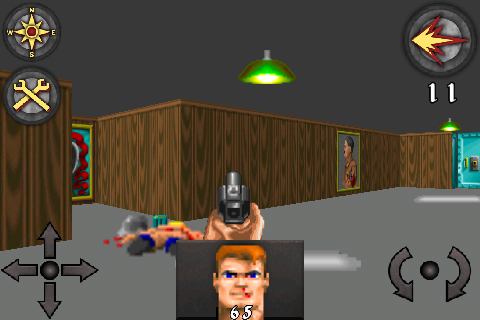
\includegraphics[width=\textwidth]{screenshots/wolf_ios2.png}
 \end{figure}
 \par
 The most notorious improvement is bilinear filtering, thanks to hardware accelerated rendering.

 Bilinear filtering is not for everybody. Some people complained the enemies were "blurry" and wanted to see the pixels.\\ Following, the release notes of Wolfenstein3D iOS on March 25, 2009:

\subsection{iPhone development}

By John Carmack, Technical Director, Id Software\\
\par

I had been frustrated for over a year with the fact that we didn't have any iPhone development projects going internally at Id.  I love my iPhone, and I think the App Store is an extremely important model for the software business.  Unfortunately, things have conspired against us being out early on the platform.\\
\par

Robert Duffy and I spent a week early on starting to bring up the Orcs \& Elves DS codebase on the iPhone, which would have been a nice project for a launch title, but it wasn't going to be a slam dunk.  The iPhone graphics hardware is a more capable superset of the DS hardware (the driver overhead is far, far worse, though), but the codebase was fairly DS specific, with lots of Nintendo API calls all over the place.  I got the basics drawing by converting things to OpenGL ES, but I was still on the fence as to whether the best approach to get all the picky little special effects working would be a complete GL conversion, or a DS graphics library emulation layer.  Coupled with the fact that the entire user interface would need to be re-thought and re-tested, it was clear that the project would take several months of development time, and need artists and designers as well as coding work.  I made the pitch that this would still be a good plan, but the idMobile team was already committed to the Wolfenstein RPG project for conventional Java and BREW mobile phones, and Anna didn't want to slip a scheduled milestone on the established, successful development directions there for a speculative iPhone project.\\
\par

After thinking about the platform's capabilities a bit more, I had a plan for an aggressive, iPhone specific project that we actually started putting some internal resources on, but the programmer tasked with it didn't work out and was let go.  In an odd coincidence, an outside development team came to us with a proposal for a similar project on the Wii, and we decided to have them work on the iPhone project with us instead.  We should be announcing this project soon, and it is cool.  It is also late, but that's software development...\\
\par

Late last year, the mobile team had finished up all the planned versions of Wolfenstein RPG, but EA had suggested that in addition to the hundreds of customized versions they normally produce for all the various mobile phones, they were interested in having another team do a significant media quality improvement on it for the iPhone.  While Wolf RPG is a very finely crafted product for traditional cell phones, it wasn't designed for the iPhone's interface or capabilities, so it wouldn't be an ideal project, but it should still be worth doing.  When we got the first build to test, I was pleased with how the high res artwork looked, but I was appalled at how slow it ran.  It felt like one of the mid range java versions, not better than the high end BREW as I expected.  I started to get a sinking feeling.  I searched around in the level for a view that would confirm my suspicion, and when I found a clear enough view of some angled geometry I saw the tell-tale mid-polygon affine swim in the texture as I rotated.  They were using the software rasterizer on the iPhone.  I patted myself on the back a bit for the fact that the combination of my updated mobile renderer, the intelligent level design / restricted movement, and the hi-res artwork made the software renderer almost visually indistinguishable from a hardware renderer, but I was very unhappy about the implementation.\\
\par

I told EA that we were NOT going to ship that as the first Id Software product on the iPhone.  Using the iPhone's hardware 3D acceleration was a requirement, and it should be easy - when I did the second generation mobile renderer (written originally in java) it was layered on top of a class I named TinyGL that did the transform / clip / rasterize operations fairly close to OpenGL semantics, but in fixed point and with both horizontal and vertical rasterization options for perspective correction.  The developers came back and said it would take two months and exceed their budget.\\
\par

Rather than having a big confrontation over the issue, I told them to just send the project to me and I would do it myself.  Cass Everitt had been doing some personal work on the iPhone, so he helped me get everything set up for local iPhone development here, which is a lot more tortuous than you would expect from an Apple product.  As usual, my off the cuff estimate of "Two days!" was optimistic, but I did get it done in four, and the game is definitely more pleasant at 8x the frame rate.\\
And I had fun doing it.\\
\par

Since we now were doing something resembling "real work" on the iPhone at the office, we kept it going at a low priority.  One of the projects Cass was tinkering around with at home was a port of Quake 3, and we talked about different interface strategies every now and then.\\
Unfortunately, when we sat down to try a few things out, we found that Q3 wasn't really running fast enough to make good judgments on iPhone control systems.  The hardware should be capable enough, but it will take some architectural changes to the rendering code to get the most out of it.\\
\par

I was just starting to set up a framework to significantly revise Q3 when I considered the possibility of just going to an earlier codebase to experiment with initially.  If we wanted to factor performance out of the equation, we could go all the way back to Wolfenstein 3D, the grandfather of FPS games.  It had the basic run and gun play that has been built on for fifteen years, but it originally ran on 286 computers, so it should be pretty trivial to hold a good framerate on the iPhone.\\
\par

Wolfenstein was originally written in Borland C and TASM for DOS, but I had open sourced the code long ago, and there were several projects that had updated the original code to work on OpenGL and modern operating systems.  After a little looking around, I found Wolf3D Redux at http://wolf3dredux.sourceforge.net/.  One of the development comments about "removal of the gangrenous 16 bit code" made me smile.\\
\par

It was nice and simple to download, extract data from a commercial copy of Wolfenstein, and start playing on a PC at high resolution.  Things weren't as smooth as they should be at first, but two little changes made a huge difference - going at VBL synced update rates with one tic per cycle instead of counting milliseconds to match 70 hz game tics, and fixing a bug with premature integralization in the angle update code that caused mouse movement to be notchier than it should be.  The game was still fun to play after all these years, and I began to think that it might be worthwhile to actually make a product out of Wolfenstein on the iPhone, rather than just using it as a testbed, assuming the controls worked out as fun to play.  The simple episodic nature of the game would make it easy to split up into a \$0.99 version with just the first episode, a more expensive version with all sixty levels, and we could release Spear of Destiny if there was additional demand.  I was getting a little ahead of myself without a fun-to-play demonstration of feasibility on the iPhone, but the idea of moving the entire line of classic Id titles over - Wolf, Doom, Quake, Quake 2, and Quake Arena, was starting to sound like a real good idea.\\
\par

I sent an email to the Wolf 3D Redux project maintainer to see if he might be interested in working on an iPhone project with us, but it had been over a year since the last update, and he must have moved on to other things.  I thought about it a bit, and decided that I would go ahead and do the project myself.  The "big projects" at Id are always top priority, but the systems programming work in Rage is largely completed, and the team hasn't been gated on me for anything in a while.  There is going to be memory and framerate optimization  work going on until it ships, but I decided that I could spend a couple weeks away from Rage to work on the iPhone exclusively.  Cass continued to help with iPhone system issues, I drafted Eric Will to create the few new art assets, and Christian Antkow did the audio work, but this was the first time I had taken full responsibility for an entire product in a very long time.\\
\par

\subsection{Design notes}

The big question was how "classic" should we leave the game?  I have bought various incarnations of Super Mario Bros on at least four Nintendo platforms, so I think there is something to be said for the classics, but there were so many options for improvement.  The walls and sprites in the game were originally all 64 x 64 x 8 bit color, and the sound effects were either 8khz / 8 bit mono or (sometimes truly awful) FM synth sounds.  Changing these would be trivial from a coding standpoint.  In the end, I decided to leave the game media pretty much unchanged, but tweak the game play a little bit, and build a new user framework around the core play experience.  This decision was made a lot easier by the fact that we were right around the 10 meg over-the-air app download limit with the converted media.  This would probably be the only Id project to ever be within hailing distance of that mark, so we should try to fit it in.\\
\par

The original in-game status bar display had to go, because the user's thumbs were expected to cover much of that area.  We could have gone with just floating stats, but I thought that BJ's face added a lot of personality to the game, so I wanted to leave that in the middle of the screen.  Unfortunately, the way the weapon graphics were drawn, especially the knife, caused issues if they were just drawn above the existing face graphics.  I had a wider background created for the face, and used the extra space for directional damage indicators, which was a nice improvement in the gameplay.  It was a tough decision to stop there on damage feedback, because a lot of little things with view roll kicks, shaped screen blends, and even double vision or blurring effects, are all pretty easy to add and quite effective, but getting farther away from "classic".\\
\par

I started out with an explicit "open door" button like the original game, but I quickly decided to just make that automatic.  Wolf and Doom had explicit "use" buttons, but we did away with them on Quake with contact or proximity activation on everything.  Modern games have generally brought explicit activation back by situationally overriding attack, but hunting for push walls in Wolf by shooting every tile wouldn't work out.  There were some combat tactics involving explicitly shutting doors that are gone with automatic-use, and some secret push walls are trivially found when you pick up an item in front of them now, but this was definitely the right decision.\\
\par

You could switch weapons in Wolf, but almost nobody actually did, except for occasionally conserving ammo with the chain gun, or challenges like "beat the game with only the knife".  That functionality didn't justify the interface clutter.\\
\par

The concept of "lives" was still in wolf, with 1-ups and extras at certain scores.  We ditched that in Doom, which was actually sort of innovative at the time, since action games on computers and consoles were still very much take-the-quarter arcade oriented.  I miss the concept of "score" in a lot of games today, but I think the finite and granular nature of the enemies, tasks, and items in Wolf is better suited to end-of-level stats, so I removed both lives and score, but added persistent awards for par time, 100\% kills, 100\% secrets, and 100\% treasures.  The award alone wasn't enough incentive to make treasures relevant, so I turned them into uncapped +1 health crumbs, which makes you always happy to find them.\\
\par

I increased the pickup radius for items, which avoided the mild frustration of having to sometimes make a couple passes at an item when you are cleaning up a room full of stuff.\\
\par

I doubled the starting ammo on a fresh level start.  If a player just got killed, it isn't good to frustrate them even more with a severe ammo conservation constraint.  There was some debate about the right way to handle death:  respawn with the level as is (good in that you can keep making progress if you just get one more shot off each time, bad in that weapon pickups are no longer available), respawn just as you entered the level (good - keep your machinegun / chaingun, bad - you might have 1 health), or, what I chose, restart the map with basic stats just as if you had started the map from the menu.\\
\par

There are 60 levels in the original Wolf dataset, and I wanted people to have the freedom to easily jump around between different levels and skills, so there is no enforcement of starting at the beginning.  The challenge is to /complete /a level, not /get to/ a level.  It is fun to start filling in the grid of level completions and awards, and it often feels better to try a different level after a death.  The only exception to the start-anywhere option is that you must find the entrance to the secret levels before you can start a new game there.\\
\par

In watching the early testers, the biggest issue I saw was people sliding off doors before they opened, and having to maneuver back around to go through.  In Wolf, as far as collision detection was concerned, everything was just a 64×64 tile map that was either solid or passable.
Doors changed the tile state when they completed opening or began closing.  There was discussion about magnetizing the view angle towards doors, or somehow beveling the areas around the doors, but it turned out to be pretty easy to make the door tiles only have a solid central core against the player, so players would slide into the "notch" with the door until it opened.  This made a huge improvement in playability.\\
\par

There is definitely something to be said for a game that loads in a few seconds, with automatic save of your position when you exit.  I did a lot of testing by playing the game, exiting to take notes in the iPhone notepad, then restarting Wolf to resume playing.  Not having to skip through animated logos at the start is nice.  We got this pretty much by accident with the very small and simple nature of Wolf, but I think it is worth specifically optimizing for in future titles.\\
\par

The original point of this project was to investigate FPS control schemes for the iPhone, and a lot of testing was done with different schemes and parameters.  I was sort of hoping that there would be one "obviously correct" way to control it, but it doesn't turn out to be the case.\\
\par

For a casual first time player, it is clearly best to have a single forward / back / turn control stick and a fire button.\\
\par

Tilt control is confusing for first exposure to the game, but I think it does add to the fun factor when you use it.  I like the tilt-to-move option, but people that play a lot of driving games on the iPhone seem to like tilt-to-turn, where you are sort of driving BJ through the levels.  Tilt needs a decent deadband, and a little bit of filtering is good.  I was surprised that the precision on the accelerometer was only a couple degrees, which makes it poorly suited for any direct mapped usage, but it works well enough as a relative speed control.\\
\par

Serious console gamers tend to take to the "dual stick" control modes easily for movement, but the placement of the fire button is problematic.  Using an index finger to fire is effective but uncomfortable.  I see many players just move the thumb to fire, using strafe movement for fine tuning aim.  It is almost tempting to try to hijack the side volume switch for fire, but the ergonomics aren't quite right, and it would be very un-Apple-like, and wouldn't be available on the iPod touch (plus I couldn't figure out how...).\\
\par

We tried a tilt-forward to fire to allow you to keep your thumbs on the dual control sticks, but it didn't work out very well.  Forward / back tilt has the inherent variable holding angle problem for anything, and a binary transition point is hard for people to hold without continuous feedback.  Better visual feedback on the current angle and trip point would help, but we didn't pursue it much.  For a game with just, say, a rocket launcher, shake/shove-to-fire might be interesting, but it isn't any good for wolf.\\
\par

It was critical for the control sticks to be analog, since digital direction pads have proven quite ineffective on touch screens due to progressive lack of registration during play.  With an analog stick, the player has continuous visual feedback of the stick position in most cases, so they can self correct.  Tuning the deadband and slide off behavior are important.\\
\par

Level design criteria has advanced a lot since Wolfenstein, but I wasn't going to open up the option of us modifying the levels, even though the start of the first level is painfully bad for a first time player, with the tiny, symmetric rooms for them to get their nose mashed into walls and turned around in.  The idea is that you started the game in a prison cell after bashing your guard over the head, but even with the exact same game tools, we would lead the player through the experience much better now.  Some of the levels are still great fun to play, and it is interesting to read Tom Hall and John Romero's designer notes in the old hint manuals, but the truth is that some levels were scrubbed out in only a couple hours, unlike the long process of testing and adjustment that goes on today.\\
\par

It was only after I thought I was basically done with the game that Tim Willits pointed out the elephant in the gameplay room - for 95\% of players, wandering around lost in a maze isn't very much fun.
Implementing an automap was pretty straightforward, and it probably added more to the enjoyment of the game than anything else.  Before adding this, I thought that only a truly negligible amount of people would actually finish all 60 levels, but now I think there might be enough people that get through them to justify bringing the Spear of Destiny levels over later.\\
\par

When I was first thinking about the project I sort of assumed that we wouldn't bother with music, but Wolf3D Redux already had code that converted the old id music format into ogg, so we would up with support at the beginning, and it turned out pretty good.  We wound up ripping the red book audio tracks from one of the later commercial Wolf releases and encoding at a different bitrate, but I probably wouldn't have bothered if not for the initial support.  It would have been nice to re-record the music with a high quality MIDI synth, but we didn't have the original MIDI source, and Christian said that the conversion back from the id music format to midi was a little spotty, and would take a fair amount of work to get right.  I emailed Bobby Prince, the original composer, to see if he had any high quality versions still around, but he didn't get back with me.\\
\par

The game is definitely simplistic by modern standards, but it still has its moments.  Getting the drop on a brown shirt just as he is pulling his pistol from the holster.  Making an SS do the "twitchy dance" with your machine gun.  Rounding a corner and unloading your weapon on … a potted plant.  Simplistic plays well on the iPhone.\\
\par

\subsection{Programming notes}
Cass and I got the game running on the iPhone very quickly, but I was a little disappointed that various issues around the graphics driver, the input processing, and the process scheduling meant that doing a locked-at-60-hz game on the iPhone wasn't really possible.  I hope to take these up with Apple at some point in the future, but it meant that Wolf would be a roughly two tick game.  It is only "roughly" because there is no swapinterval support, and the timer scheduling has a lot of variability in it.  It doesn't seem to matter all that much, the play is still smooth and fun, but I would have liked to at least contrast it with the perfect limit case.\\
\par

It turns out that there were a couple issues that required work even at 30hz.  For a game like Wolf, any PC that is in use today is essentially infinitely fast, and the Wolf3D Redux code did some things that were convenient but wasteful.  That is often exactly the right thing to do, but the iPhone isn't quite as infinitely fast as a desktop PC.\\
\par

Wolfenstein (and Doom) originally drew the characters as sparse stretched columns of solid pixels (vertical instead of horizontal for efficiency in interleaved planar mode-X VGA), but OpenGL versions need to generate a square texture with transparent pixels.  Typically this is then drawn by either alpha blending or alpha testing a big quad that is mostly empty space.  You could play through several early levels of Wolf without this being a problem, but in later levels there are often large fields of dozens of items that stack up to enough overdraw to max out the GPU and drop the framerate to 20 fps.  The solution is to bound the solid pixels in the texture and only draw that restricted area, which solves the problem with most items, but Wolf has a few different heavily used ceiling lamp textures that have a small lamp at the top and a thin but full width shadow at the bottom.  A single bounds doesn't exclude many texels, so I wound up including two bounds, which made them render many times faster.\\
\par

The other problem was CPU related.  Wolf3d Redux used the original ray casting scheme to find out which walls were visible, then called a routine to draw each wall tile with OpenGL calls.  The code looked something like this:\\
\par
\begin{minipage}{\textwidth}
\lstinputlisting[language=C]{code/wolfesntesin3d_iOS_codesample1.c}
\end{minipage}
\par

I winced when I saw that at the top of the instruments profile, but again, you could play all the early levels that only had twenty or thirty visible tiles at a time without it actually being a problem. \\
\par

However, some later levels with huge open areas could have over a hundred visible tiles, and that led to 20hz again.  The solution was a trivial change to something resembling:\\
\par

\begin{minipage}{\textwidth}
\lstinputlisting[language=C]{code/wolfesntesin3d_iOS_codesample2.c}
\end{minipage}
\par

Wolf3D Redux included a utility that extracted the variously packed media from the original games and turned them into cleaner files with modern formats.  Unfortunately, an attempt at increasing the quality of the original art assets by using hq2x graphics scaling to turn the 64x64 art into better filtered 128×128 arts was causing lots of sprites to have fringes around them due to incorrect handling of alpha borders.  It wasn't possible to fix it up at load time, so I had to do the proper outline-with-color-but-0-alpha operations in a modified version of the extractor.  I also decided to do all the format conversion and mip generation there, so there was no significant CPU time spent during texture loading, helping to keep the load time down.  I experimented with the PVRTC formats, but while it would have been ok for the walls, unlike with DXT you can't get a lossless alpha mask out of it, so it wouldn't have worked for the sprites.  Besides, you really don't want to mess with the carefully chosen pixels in a 64x64 block very much when you scale it larger than the screen on occasion.\\
\par

I also had to make one last minute hack change to the original media - the Red Cross organization had asserted their trademark rights over red crosses (sigh) some time after we released the original Wolfenstein 3D game, and all new game releases must not use red crosses on white backgrounds as health symbols.  One single, solitary sprite graphic got modified for this release.\\
\par

User interface code was the first thing I started making other programmers do at Id when I no longer had to write every line of code in a project, because I usually find it tedious and unrewarding.  This was such a small project that I went ahead and did it myself, and I learned an interesting little thing.  Traditionally, UI code has separate drawing and input processing code, but on a touchscreen device, it often works well to do a combined "immediate mode interface", with code like this:\\
\par
\begin{minipage}{\textwidth}
\lstinputlisting[language=C]{code/wolfesntesin3d_iOS_codesample3.c}
\end{minipage}
\par
Doing that for the floating user gameplay input controls would introduce a frame of response latency, but for menus and such, it works very well.\\
\par

One of the worst moments during the development was when I was getting ready to hook up the automatic savegame on app exit.  There wasn't any savegame code.  I went back and grabbed the original 16 bit dos code for load / save game, but when I compiled I found out that the Wolf3d Redux codebase had changed a lot more than just the near / far pointer issues, asm code, and comment blocks.  The changes were sensible things, like grouping more variables into structures and defining enums for more things, but it did mean that I wasn't dealing with the commercially tested core that I thought I was.  It also meant that I was a lot more concerned about a strange enemy lerping through the world bug I had seen a couple times.\\
\par

I seriously considered going back to the virgin codebase and reimplementing the OpenGL rendering from scratch.  The other thing that bothered me about the Redux codebase was that it was basically a graft of the Wolf3D code into the middle of a gutted Quake 2 codebase.  This was cool in some ways, because it gave us a console, cvars, and the system / OpenGL portable framework, and it was clear the original intention was to move towards multiplayer functionality, but it was a lot of bloat.  The original wolf code was only a few dozen C files, while the framework around it here was several times that.\\
\par

Looking through the original code brought back some memories.  I stopped signing code files years ago, but the top of WL\_MAIN.C made me smile:\\
\par
\begin{minipage}{\textwidth}
\lstinputlisting[language=C]{code/wolfesntesin3d_iOS_codesample4.c}
\end{minipage}
\par
It wasn't dated, but that would have been in 1991.\\
\par

In the end, I decided to stick with the Redux codebase, but I got a lot more free with hacking big chunks of it out.  I reimplemented load / save game (fixing the inevitable pointer bugs involved), and by littering asserts throughout the code, I tracked the other problem down to an issue with making a signed comparison against one of the new enum types that compare as unsigned.  I'm still not positive if this was the right call, since the codebase is sort of a mess with lots of vestigial code that doesn't really do anything, and I don't have time to clean it all up right now.\\
\par

Of course, someone else is welcome to do that.  The full source code for the commercial app is available on the web site.  There was a little thought given to the fact that if I had reverted to the virgin source, the project wouldn't be required to be under the GPL.  Wolf and the app store presents a sort of unique situation - a user can't just compile the code and choose not to pay for the app, because most users aren't registered developers, and the data isn't readily available, but there is actually some level of commercial risk in the fast-moving iPhone development community.  It will not be hard to take the code that is already fun to play, pull a bunch of fun things off the net out of various projects people have done with the code over the years, dust off some old map editors, and load up with some modern quality art and sound.\\
\par

Everyone is perfectly within their rights to go do that, and they can aggressively try to bury the original game if they want.  However, I think there is actually a pretty good opportunity for cooperation.  If anyone makes a quality product and links to the original Wolf app, we can start having links to "wolf derived" or "wolf related" projects.\\
That should turn out to be a win for everyone.\\
\par

I'm going back to Rage for a while, but I do expect Classic Doom to come fairly soon for the iPhone.\\
\par

 






 

\section{ShadowCaster}
Developed by Raven with a licensed technology from id software. John Carmack wrote the ShadowCaster 3D engine during his technology research after id Software completed Wolfenstein 3D. The engine features diminished lighting, texture mapped floors and ceilings, walls with variable heights and sloped floors. The map are still made of blocks with ortogonal walls. The engine was "about half as fast as that of Wolfenstein" but fit the exploration of ShadowCaster rather than the fast paced action of Doom.

\begin{figure}[H]
\centering
 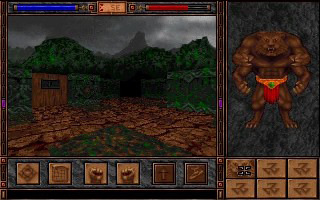
\includegraphics[width=\textwidth]{screenshots/shadowcaster.png}
 \end{figure}
 \par



\end{document}
